%!TEX root = ./template-skripsi.tex
%-------------------------------------------------------------------------------
%                            BAB VI
%               		HASIL DAN PEMBAHASAN
%-------------------------------------------------------------------------------

\chapter{HASIL DAN PEMBAHASAN}
	\section{Proses Pengembangan Sistem dengan Metode \emph{Extreme Programming}}
	Sistem informasi penggajian karyawan ini dikembangkan dengan menggunakan metode \emph{Extreme Programming} (XP). Alasan peneliti menggunakan metode tersebut dikarenakan metode XP mudah dan fleksibel terhadap adanya perubahan kebutuhan sistem selama masa pengembangan. Dengan menggunakan metode XP ini peneliti melakukan empat tahapan selama masa pengembangan, yaitu \emph{planning}, \emph{design}, \emph{coding}, dan \emph{testing}.
	
	\subsection{Pengembangan Sistem Siklus 1}
	
	\subsubsection{\emph{Planning} Siklus 1}
	Pada tahap \emph{planning} siklus pertama ini peneliti melakukan analisis kebutuhan dari sistem yang dikembangkan. Analisis tersebut dilakukan dengan cara wawancara dan diskusi dengan pihak Universitas Proklamasi 45 selaku \emph{project owner}. Hasil yang didapat adalah siapa saja yang akan menggunakan sistem nantinya, dan bagaimana sistem tersebut bekerja.
	
	Sistem yang dikembangkan nantinya memiliki enam pengguna, yaitu staf SDM, staf Akademik, staf Keuangan, pimpinan, kepala unit, dan karyawan. Penjelasan mengenai pengguna tersebut adalah sebagai berikut:
	\begin{enumerate}
	    \itemsep0em
	    \item Staf SDM
	    
	    Pengguna ini memiliki wewenang dalam melakukan manajemen unit kerja dan jabatan, periode kerja dan jam kerja karyawan, data karyawan, data lembur dan rapat, serta data absensi karyawan.
	    \item Staf Akademik
	    
	    Pengguna ini memiliki hak akses atau wewenang dalam melakukan manajemen data ujian yang meliputi input data ujian, data pengawas ujian, dan data korektor ujian.
	    \item Staf Keuangan
	    
	    Pengguna ini memiliki hak akses atau wewenang dalam melakukan \emph{generate} slip gaji karyawan dan mencetak laporan penggajian. Selain itu juga dapat melakukan validasi upah selain gaji pokok seperti upah lembur, upah rapat, upah pengawas ujian dan upah korektor ujian.
	    \item Pimpinan
	    
	    Pimpinan yang dimaksud disini adalah pihak Yayasan Universitas Proklamasi 45, yang memiliki hak akses untuk melihat laporan penggajian karyawan.
	    
	    \item Kepala Unit
	    
	    Kepala unit memiliki hak akses atau wewenang dalam melakukan input data insentif operasional karyawan yang dibawahinya.
	    \item Karyawan
	    
	    Karyawan yang dimaksud disini adalah pengguna biasa yang hanya memiliki akses untuk melihat data rekap absensi, data rapat, data lembur, data pengawas, dan data korektor yang berhubungan dengan karyawan tersebut. Karyawan juga dapat melihat rincian gaji dan mencetak slip gaji.
	\end{enumerate}
	
	Sistem informasi penggajian yang dikembangkan nantinya akan memiliki alur atau proses yang terstruktur dengan baik. Dimulai dari staf SDM melakukan penginputan periode kerja, pengunggahan data absensi, menambahkan data lembur karyawan, menambahkan data rapat dan melakukan perekapan data tersebut. Kemudian staf Akademik melakukan penambahan data ujian, data pengawas dan korektor ujian serta melakukan perekapan data tersebut. Kepala unit dalam sistem yang dikembangkan bertugas mengisi data insentif operasional karyawan. Semua data yang telah disebutkan merupakan komponen dari penggajian. Setelah semua data berhasil direkap, staf Keuangan dapat melakukan \emph{generate} slip gaji dan mencetak laporan penggajian. Pihak pimpinan atau yayasan dapat melihat laporan penggajian sebagai bahan evaluasi.
	
	\subsubsection{\emph{Design} Siklus 1}
	Pada \emph{design} siklus pertama ini peneliti membuat perancangan proses berupa \emph{use case diagram} berdasarkan hasil analisis yang telah dilakukan. Tujuan pembuatan \emph{use case diagram} adalah untuk menggambarkan fitur atau fungsi apa saja yang dimiliki oleh sistem yang dikembangkan. \emph{Use case diagram} pada siklus pertama ini dapat dilihat pada Gambar \ref{use_case_pertama}.
	\begin{figure}[H]
	    \centering            		    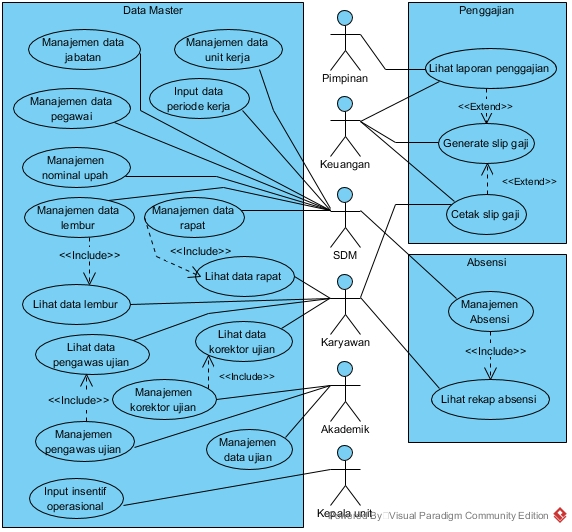
\includegraphics[width=10cm]{gambar/use-case-pertama}
	    \caption{\emph{Use Case Diagram} Siklus Pertama}
	    \label{use_case_pertama}
	\end{figure}
	Perbedaan dengan \emph{Use Case Diagram} pada Gambar \ref{usecase} adalah pada siklus pertama ini berfokus pada fungsionalitas utama dari sistem yang dikembangkan. Fungsionalitas utama tersebut adalah pengelolaan data master, data absensi, data upah selain gaji pokok, dan generate slip gaji karyawan.
	
	\subsubsection{\emph{Coding} Siklus 1}
	Pada tahap \emph{coding} siklus pertama ini peneliti mulai melakukan pembuatan sistem berdasarkan hasil rancangan (\emph{design}) sebelumnya. Pertama-tama peneliti mengimplementasikan pembuatan fungsi \emph{login} sesuai dengan hak akses pengguna masing-masing. Dalam mengimplementasikan pembuatan fitur pada sistem, peneliti menyelesaikan fitur untuk masing-masing pengguna terlebih dahulu, yang dapat dijelaskan sebagai berikut:
	\begin{enumerate}
	    \itemsep0em
	    \item Fitur untuk Staf SDM
	    
	    Untuk staf SDM, peneliti memulai dengan mengimplementasikan pembuatan fitur manajemen data periode kerja, karena periode kerja nantinya akan menjadi parameter dari setiap proses penambahan data di dalam sistem. Kemudian berlanjut dengan pembuatan fitur manajemen jam kerja, manajemen data unit kerja dan jabatan, manajemen data karyawan, manajemen data absensi, manajemen data lembur dan manajemen data rapat.
	    
	    Pada siklus pertama ini ketika staf SDM ingin melakukan proses \emph{upload} absensi, perlu memilih periode kerja dan memilih \emph{file Excel} yang berisikan data absensi karyawan. Nantinya sistem akan membaca data pada \emph{file Excel} tersebut dan menyimpannya ke dalam \emph{database}. \emph{Source code} untuk fitur \emph{upload} absensi dapat dilihat pada Gambar \ref{coding_abs_satu}, Gambar \ref{coding_abs_dua} dan Gambar \ref{coding_abs_tiga}.
	    \begin{figure}[H]
	    \centering            		    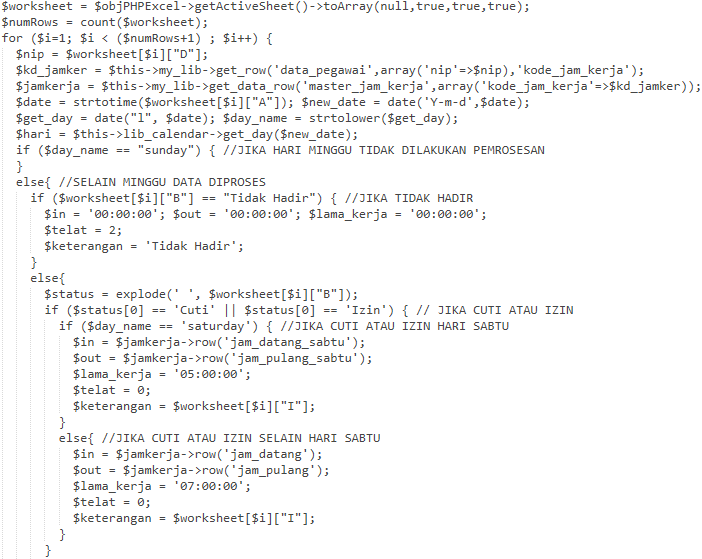
\includegraphics[width=13cm]{gambar/coding/up-absensi1-siklus1}
	    \caption{\emph{Source Code Upload} Absensi Bagian-1 Siklus Pertama}
	    \label{coding_abs_satu}
    	\end{figure}
    	\begin{figure}[H]
    	    \centering            		    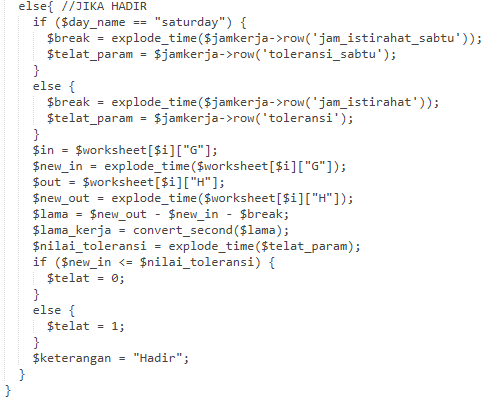
\includegraphics[width=10cm]{gambar/coding/up-absensi2-siklus1}
    	    \caption{\emph{Source Code Upload} Absensi Bagian-2 Siklus Pertama}
    	    \label{coding_abs_dua}
    	\end{figure}
    	\begin{figure}[H]
    	    \centering            		    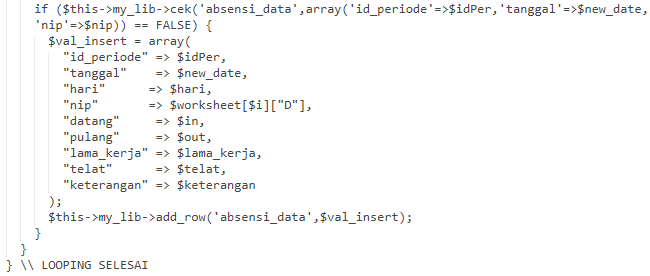
\includegraphics[width=11cm]{gambar/coding/up-absensi3-siklus1}
    	    \caption{\emph{Source Code Upload} Absensi Bagian-3 Siklus Pertama}
    	    \label{coding_abs_tiga}
    	\end{figure}
	    \item Fitur untuk Staf Akademik
	    
	    Implementasi fitur untuk staf Akademik ini peneliti mulai dari pembuatan fitur manajemen data ujian terlebih dahulu, kemudian berlanjut dengan fitur manajemen data pengawas ujian dan data korektor ujian. Hal itu dikarenakan apabila staf Akademik ingin mengisi data pengawas dan korektor ujian, terlebih dahulu harus sudah ada data ujian.
	    \item Fitur untuk Kepala Unit
	    
	    Untuk fitur Kepala Unit, peneliti mengimplementasikan fitur pemberian insentif operasional kepada karyawan. Pada siklus pertama ini, Kepala Unit hanya memiliki satu fitur tersebut. 
	    \item Fitur untuk Staf Keuangan
	    
	    Setelah fitur staf SDM, staf Akademik dan Kepala Unit selesai diimplementasikan, yang dimana terdapat proses manajemen data-data komponen penggajian, peneliti berlanjut dengan membuat fitur \emph{generate} slip gaji untuk staf Keuangan. Kemudian selanjutnya adalah membuat fitur lihat laporan penggajian.
	    \item Fitur untuk Pimpinan/ Yayasan
	    
	    Fitur untuk pimpinan/ yayasan ini hanya melihat laporan penggajian, sehingga peneliti dapat menggunakan kembali \emph{source code} pada fitur lihat laporan penggajian yang sebelumnya dibuat untuk staf Keuangan.
	    \item Fitur untuk Karyawan
	    
	    Implementasi fitur untuk karyawan pada siklus pertama ini hanya sebatas melihat data yang meliputi data rekap absensi, data lembur, data rapat, data pengawas dan korektor ujian. Seluruh data tersebut sudah ditambahkan oleh staf SDM dan staf Akademik, sehingga peneliti hanya perlu menampilkannya untuk masing-masing karyawan. Kemudian berlanjut dengan membuat fitur cetak slip gaji untuk karyawan.
	\end{enumerate}
	
	
	
	\subsubsection{\emph{Testing} Siklus 1}
	Pada tahap \emph{testing} siklus pertama ini peneliti melibatkan semua pengguna sistem dan berfokus pada fungsionalitas terhadap sistem yang dikembangkan. Selama proses \emph{testing} tersebut peneliti mendapatkan permintaan penambahan beberapa fitur baru yang dapat dilihat pada Tabel \ref{testing_siklus_pertama}.
	\begin{spacing}{1.25}
	\begin{longtable}{|>{\centering}p{1.5em}|>{\raggedright}p{8cm}|p{3cm}|}
        \caption{Penambahan Fitur Baru} 
	    \label{testing_siklus_pertama} \\
        \hline
        \textbf{No.} & \centering \textbf{Fitur Baru} & \textbf{Aktor} \\
        \hline 
        \endfirsthead
        \multicolumn{3}{c}{{\bfseries \tablename\ \thetable{}: }Penambahan Fitur Baru (lanjutan)} \\
        \hline
        \textbf{No.} & \centering \textbf{Fitur Baru} & \textbf{Aktor} \\ \hline
        \endhead
        \hline \multicolumn{3}{|r|}{{Berlanjut halaman selanjutnya}} \\ \hline
        \endfoot
        \hline \hline
        \endlastfoot
        1. & \emph{Input field} pilih tanggal \emph{enable} setelah periode kerja dipilih serta \emph{min} dan \emph{max} tanggal tersebut sesuai dengan periode kerja & SDM \\ \hline
        2. & Rekap absensi otomatis & SDM \\ \hline
        3. & Mengubah data absensi karyawan & SDM \\ \hline
        4. & Pengajuan lembur oleh karyawan & Karyawan \\ \hline
	    5. & Memperpendek proses \emph{generate} slip gaji karyawan & Keuangan \\ \hline
	    
	\end{longtable}
    \end{spacing}
    \vspace{4mm}
	
\subsection{Pengembangan Sistem Siklus 2}
Pada siklus kedua ini, terdapat perbedaan yang mendasar dengan siklus sebelumnya, yaitu lebih berfokus pada peningkatan kinerja sistem. Hal ini dapat dilihat dari hasil pengujian siklus pertama. Penjelasan lebih detailnya akan dibahas dalam tahapan siklus kedua ini.
	
	\subsubsection{\emph{Planning} Siklus 2}
	Pada tahap \emph{planning} siklus kedua ini peneliti kembali melakukan analisis berdasarkan hasil \emph{testing} siklus pertama. Hasil analisis tersebut adalah penambahan fungsionalitas sistem seperti yang tertera pada Tabel \ref{testing_siklus_pertama}.
	
	Tujuan dari perubahan cara kerja \emph{input field} pilih tanggal adalah agar tanggal yang diinputkan tidak kurang ataupun tidak lebih dari batas awal dan batas akhir periode kerja yang dipilih. Sehingga sebelum periode kerja dipilih, \emph{input field} pilih tanggal dalam keadaan \emph{disable}. Hal tersebut merupakan langkah efektif agar data yang dimasukkan ke dalam sistem lebih terdokumentasi dengan benar dan rapi berdasarkan periode kerjanya.
	
	Selanjutnya maksud dari penambahan fungsionalitas rekap absensi otomatis adalah ketika staf SDM melakukan \emph{upload file} absensi, sistem akan membaca dan menyimpan data absensi ke dalam \emph{table} data absensi, sekaligus melakukan perekapan data absensi tersebut yang kemudian akan disimpan ke dalam \emph{table} rekap absensi. Hal ini akan berdampak terhadap kinerja sistem ketika melakukan proses \emph{generate} slip gaji karyawan, karena proses \emph{generate} slip gaji tersebut membutuhkan data rekap absensi bulanan dari masing-masing karyawan. Ketika proses \emph{generate} slip gaji, sistem cukup membaca data rekap absensi dari dalam \emph{table} rekap absensi, tidak perlu lagi melakukan kalkulasi atau perhitungan data absensi harian
	dari dalam \emph{table} data absensi.
	
	\subsubsection{\emph{Design} Siklus 2}
	Hasil analisis pada tahap \emph{planning} siklus kedua peneliti gunakan untuk melakukan penambahan dan perubahan \emph{use case diagram}, \emph{activity diagram}, \emph{sequence diagram}, \emph{database} serta rancangan antarmuka sistem.
	
	Penambahan dan perubahan yang dilakukan diantaranya adalah merancang tabel baru pada \emph{database}, yaitu tabel rekap absensi serta merubah rancangan tabel data lembur karyawan. Kemudian melakukan perancangan antarmuka untuk halaman ubah data absensi dan halaman pengajuan lembur untuk karyawan.
	
	\subsubsection{\emph{Coding} Siklus 2}
	Pada tahap \emph{coding} siklus kedua ini peneliti mengimplementasikan perubahan dan penambahan fitur dan fungsi pada sistem sesuai dengan hasil \emph{planning} dan \emph{design} siklus kedua. Pertama peneliti mengimplementasikan fungsi \emph{enable disable} dan \emph{min max} pada \emph{input field} pilih tanggal untuk setiap \emph{form} tambah data lembur, data rapat, dan data ujian. \emph{Source code} untuk mengatur \emph{input field} pilih tanggal tersebut dapat dilihat pada Gambar \ref{coding_js_gettanggal} dan Gambar \ref{coding_gettanggal}.
	\begin{figure}[H]
	    \centering            		    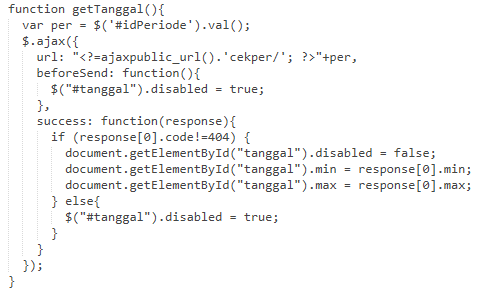
\includegraphics[width=10cm]{gambar/coding/js-get-tanggal}
	    \caption{\emph{Source Code Javascript Input Field} Pilih Tanggal}
	    \label{coding_js_gettanggal}
    \end{figure}
    \begin{figure}[H]
	    \centering            		    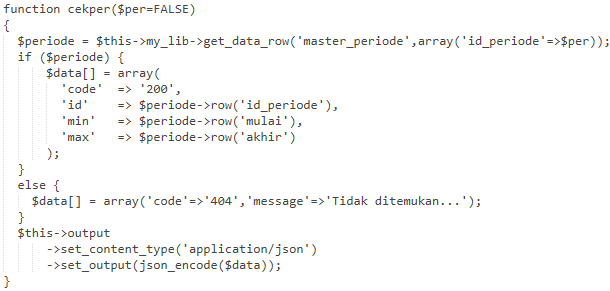
\includegraphics[width=13cm]{gambar/coding/get-tanggal}
	    \caption{\emph{Source Code} Ambil Batas Awal dan Akhir Periode Kerja}
	    \label{coding_gettanggal}
    \end{figure}
	
	Setelah itu peneliti berlanjut dengan mengimplementasikan perubahan dan penambahan fungsi rekap absensi otomatis ketika staf SDM melakukan \emph{upload} absensi dan fungsi mengubah data absensi karyawan tertentu. \emph{Source code} rekap absensi otomatis diletakkan setelah baris \emph{source code upload} absensi. \emph{Source code} dari fungsi rekap absensi dapat dilihat pada Gambar \ref{coding_rekap_absensi}.
	\begin{figure}[H]
	    \centering            		    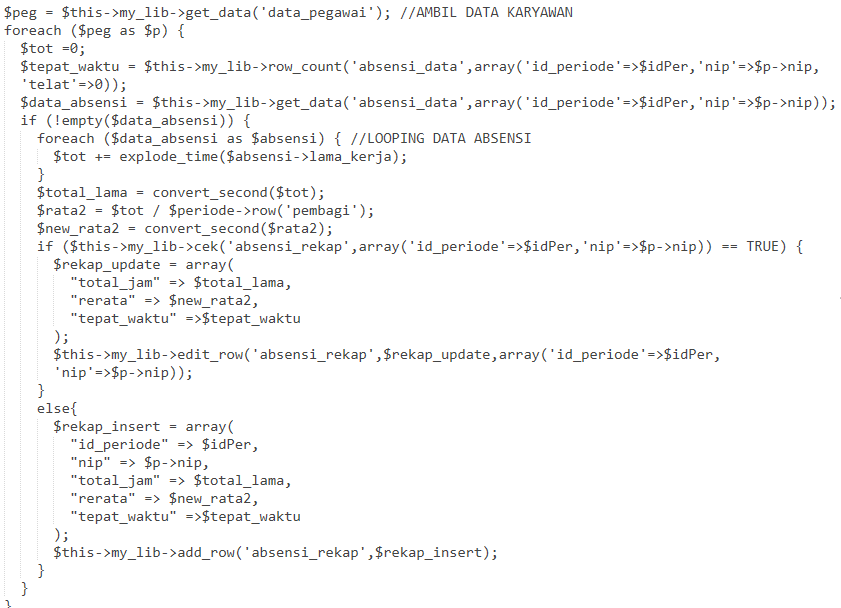
\includegraphics[width=14cm]{gambar/coding/rekap-absensi}
	    \caption{\emph{Source Code} Rekap Absensi}
	    \label{coding_rekap_absensi}
    \end{figure}
	
	\subsubsection{\emph{Testing} Siklus 2}
	Peneliti pada siklus kedua ini kembali melakukan \emph{testing} yang melibatkan pihak Universitas Proklamasi 45 selaku \emph{project owner}, khususnya staf SDM yang pada tahap \emph{testing} siklus pertama terdapat beberapa perubahan dan penambahan fitur. Hasil pengujian dari fitur yang diubah dan fitur yang baru ini tidak mendapatkan koreksi karena telah sesuai dengan permintaan sebelumnya.
	
	Selain itu, pada tahap ini peneliti juga memastikan bahwa kebutuhan dari sistem yang dikembangkan telah terpenuhi semuanya, dengan meminta seluruh aktor yang terlibat dalam sistem untuk melakukan pengujian kembali sesuai dengan hak akses atau wewenangnya masing-masing. Hasilnya, pada tahap \emph{testing} siklus kedua ini terdapat permintaan penambahan fitur baru, diantaranya adalah:
	\begin{enumerate}
	    \itemsep0em
	    \item Penambahan fitur manajemen laporan kerja karyawan untuk aktor karyawan, yang nantinya dapat digunakan untuk membuat rencana kerja harian, laporan kerja harian, checklist bulanan, dan laporan kerja harian.
	    \item Penambahan fitur penilaian kinerja karyawan untuk aktor kepala unit.
	\end{enumerate}
	
	\subsection{Pengembangan Sistem Siklus 3}
	Pada siklus ketiga ini, pengembangan lebih lanjut dilakukan terhadap sistem dengan menambahkan beberapa fitur baru berdasarkan permintaan \emph{project owner}. Fitur tersebut dianggap efektif oleh \emph{project owner} apabila diterapkan ke dalam sistem karena juga masuk sebagai salah satu faktor yang mempengaruhi besaran penggajian karyawan. Penjelasan lebih detailnya akan dibahas dalam tahapan pada siklus ketiga ini.
	
	\subsubsection{\emph{Planning} Siklus 3}
	Pada tahap \emph{planning} siklus ketiga ini peneliti kembali melakukan analisis berdasarkan hasil \emph{testing} siklus kedua. Hasil analisis tersebut adalah penambahan fungsionalitas sistem seperti yang telah dijelaskan pada tahap \emph{testing} siklus kedua.
	
	Alasan adanya penambahan fitur manajemen laporan kerja karyawan dan fitur penilaian kinerja karyawan adalah sebagai parameter dan juga acuan yang dipakai oleh Kepala Unit dalam memberikan insentif operasional kepada karyawan yang dibawahinya. Selain itu pada sistem yang berjalan saat ini, karyawan membuat laporan kerja menggunakan \emph{Microsoft Excel} yang kemudian mengirimkannya kepada Kepala Unit melalui email. Kepala Unit harus membuka satu per satu \emph{file} laporan kerja yang dikirimkan kepadanya ketika ingin melihat dan mengecek seperti apa laporan kerja karyawan tersebut. Hal tersebut akan memakan waktu yang cukup lama.
	
	\subsubsection{\emph{Design} Siklus 3}
	Pada tahap ini peneliti kembali melakukan perancangan \emph{activity diagram} dan \emph{sequence diagram} untuk manajemen laporan kerja karyawan dan penilaian kinerja karyawan. Selain itu juga membuat tabel baru pada \emph{database}, yaitu tabel rencana dan laporan kerja harian, tabel detail rencana dan laporan kerja harian, tabel checklist dan laporan bulanan, tabel detail checklist dan laporan bulanan, serta tabel penilaian kinerja karyawan. Kemudian berlanjut dengan melakukan perancangan antarmuka untuk halaman manajemen laporan kerja karyawan yang meliputi halaman buat rencana kerja harian, halaman buat laporan harian, halaman buat checklist bulanan, dan halaman buat laporan bulanan. Halaman tersebut nantinya digunakan oleh aktor karyawan.
	
	\subsubsection{\emph{Coding} Siklus 3}
	Berdasarkan hasil rancangan pada tahap \emph{design} siklus ketiga, peneliti kemudian mengimplementasikan penambahan fitur pada sistem yang dikembangkan. Yang pertama adalah mengimplementasikan fitur manajemen laporan kerja untuk aktor karyawan dengan membuat halaman buat rencana dan laporan kerja harian, serta halaman buat checklist dan laporan bulanan. Implementasi halaman tersebut dapat dilihat pada Gambar \ref{imp_hal_tambah_rkh} dan Gambar \ref{imp_hal_tambah_lh}.
	
	Setelah itu peneliti berlanjut dengan mengimplementasikan fitur lihat laporan kerja karyawan untuk aktor kepala unit yang dapat dilihat pada Gambar \ref{imp_hal_data_rkhlh} dan Gambar \ref{imp_hal_lihat_lh}. Selanjutnya adalah mengimplementasikan halaman input penilaian kinerja karyawan untuk aktor kepala unit.
	
	\subsubsection{\emph{Testing} Siklus 3}
	Setelah mengimplementasikan penambahan fitur di tahap sebelumnya, peneliti melakukan pengujian sistem kembali bersama pihak Universitas Proklamasi 45 selaku \emph{project owner}. Hasil pengujian siklus ketiga ini sudah sesuai dengan perencanaan yang telah peneliti lakukan sebelumnya, dan \emph{output} yang dihasilkan sesuai dengan permintaan \emph{project owner}. Oleh karena itu sistem yang dikembangkan telah siap untuk \emph{release}.
	
	\section{Hasil Pengujian Sistem}
	Pengujian pada sistem yang dikembangkan ini melibatkan beberapa responden selaku aktor yang terlibat di dalam sistem.
	
	\subsection{Hasil Pengujian \emph{Alpha}}
	Seluruh item uji yang peneliti rancang sebelumnya, telah dilakukan pengujian oleh seluruh aktor yang terlibat dalam sistem. Hasil pengujian \emph{alpha} ini dinyatakan berhasil karena seluruh fungsionalitas sistem dapat berjalan dengan baik.
	
	\subsection{Hasil Pengujian \emph{Beta}}
	Hasil pengujian fungsionalitas dapat dilihat pada Tabel \ref{hasil_pengujian_fungsi}, sedangkan untuk hasil pengujian usabilitas dapat dilihat pada Tabel \ref{hasil_pengujian_usa}.
	    \begin{spacing}{1.25}
	    \begin{longtable}{|>{\centering}p{1.5em}|>{\raggedright}p{7.5cm}|>{\centering}p{1cm}|>{\centering}p{1.5cm}|p{1cm}|}
    	    \caption{Hasil Pengujian Beta Fungsionalitas} 
	        \label{hasil_pengujian_fungsi} \\
            \hline
            \textbf{No.} & \centering \textbf{Pernyataan} & \textbf{YA} & \textbf{TIDAK} & \textbf{(\%)} \\
            \hline 
            \endfirsthead
            \multicolumn{5}{c}{{\bfseries \tablename\ \thetable{}: }Hasil Pengujian Beta Fungsionalitas (lanjutan)} \\
            \hline
            \textbf{No.} & \centering \textbf{Pernyataan} & \textbf{YA} & \textbf{TIDAK} & \textbf{(\%)} \\ \hline
            \endhead
            \hline \multicolumn{5}{|r|}{{Berlanjut halaman selanjutnya}} \\ \hline
            \endfoot
            \hline \hline
            \endlastfoot
            1. & Sistem dapat melakukan validasi \emph{username}, \emph{password}, hak akses ketika login, dan menampilkan menu-menu sesuai hak aksesnya & 5 & 0 & 100\% \\ \hline
	        2. & Sistem dapat melakukan fungsi manajemen data penggajian seperti tambah, edit, hapus, dan lihat detail & 5 & 0 & 100\% \\ \hline
	        3. & Sistem dapat menampilkan data-data berdasarkan periode kerja yang dipilih & 5 & 0 & 100\% \\ \hline
	        4. & Sistem dapat melakukan \emph{generate} data rekap absensi menjadi format PDF & 5 & 0 & 100\% \\ \hline
	        5. & Sistem dapat menampilkan pesan kesalahan apabila data yang dimasukkan tidak valid & 5 & 0 & 100\% \\ \hline
	        6. & Sistem dapat menampilkan rincian gaji karyawan sebelum melakukan \emph{generate} slip gaji & 5 & 0 & 100\% \\ \hline
	        7. & Untuk Kepala Unit, sistem dapat menampilkan karyawan yang dibawahi olehnya & 5 & 0 & 100\% \\ \hline
		\end{longtable}
    	\end{spacing}
    	\vspace{4mm}
    	
    Berdasarkan hasil pengujian \emph{beta} fungsionalitas pada Tabel \ref{hasil_pengujian_fungsi} yang melibatkan beberapa karyawan di lingkungan Universitas Proklamasi 45 Yogyakarta, dapat disimpulkan bahwa seluruh fitur pada sistem dapat berjalan dengan baik, dengan dibuktikan persentase hasil pengujian yang mencapai 100\%.
    	
    	\begin{spacing}{1.25}
    	\begin{longtable}{|>{\centering}p{1.5em}|>{\raggedright}p{6.5cm}|>{\centering}p{0.75cm}|>{\centering}p{0.75cm}|>{\centering}p{0.75cm}|>{\centering}p{0.75cm}|p{0.75cm}|}
    	    \caption{Hasil Pengujian Beta Usabilitas} 
	        \label{hasil_pengujian_usa} \\
            \hline
            \textbf{No.} & \centering \textbf{Pernyataan} & \textbf{SS} & \textbf{S} & \textbf{N} & \textbf{TS} & \textbf{STS} \\
            \hline 
            \endfirsthead
            \multicolumn{7}{c}{{\bfseries \tablename\ \thetable{}: }Hasil Pengujian Beta Usabilitas (lanjutan)} \\
            \hline
            \textbf{No.} & \centering \textbf{Pernyataan} & \textbf{SS} & \textbf{S} & \textbf{N} & \textbf{TS} & \textbf{STS} \\ \hline
            \endhead
            \hline \multicolumn{7}{|r|}{{Berlanjut halaman selanjutnya}} \\ \hline
            \endfoot
            \hline \hline
            \endlastfoot
            1. & Tampilan sistem menarik dan \emph{user friendly} & 4 & 1 & 0 & 0 & 0 \\ \hline
            2. & Proses pengolahan data dalam sistem berjalan dengan cepat & 1 & 3 & 1 & 0 & 0 \\ \hline
            3. & Fitur dalam sistem mudah digunakan dan dipahami & 3 & 2 & 0 & 0 & 0 \\ \hline
            4. & Bahasa yang digunakan dalam sistem mudah dipahami & 4 & 1 & 0 & 0 & 0 \\ \hline
            \multicolumn{2}{|c|}{\textbf{TOTAL}} & 12 & 7 & 1 & 0 & 0 \\ \hline
            \multicolumn{2}{|c|}{\textbf{PERSENTASE (\%)}} & 60\% & 35\% & 5\% & 0\% & 0\% \\ \hline
    	\end{longtable}
    	\end{spacing}
    	
    Berdasarkan hasil pengujian \emph{beta} usabilitas pada Tabel \ref{hasil_pengujian_usa} dapat disimpulkan bahwa responden puas dengan sistem yang dikembangkan. Hal ini dibuktikan dengan sebanyak 65\% responden yang menyatakan sangat setuju, 35\% menyatakan setuju, dan 5\% menyatakan netral.
    
    \subsection{Kesimpulan Pengujian}
    Hasil dan kesimpulan pengujian secara umum membuktikan bahwa sistem yang dikembangkan baik dari segi fungsionalitas maupun usabilitas telah lolos uji dan dapat berfungsi sesuai dengan yang diharapkan serta telah memenuhi tujuan awal pengembangan.
    
\section{Efektivitas dan Efisiensi dari Penggunaan Sistem}
Sistem informasi penggajian yang dirancang telah sesuai dengan hasil yang diharapkan oleh \emph{project owner}, yaitu dapat membantu proses penggajian yang ada di Universitas Proklamasi 45. Sistem dapat digunakan dengan baik untuk melakukan proses manajemen data penggajian, serta melihat detail atau rincian dari data penggajian. Sistem juga berhasil melakukan kalkulasi data-data komponen penggajian yang telah dimasukkan sebelumnya ketika dilakukan proses \emph{generate} slip gaji karyawan, serta dapat menampilkan rincian dari slip gaji tersebut.
    
    Proses penggajian karyawan yang berjalan sebelumnya mengharuskan dilakukannya pekerjaan atau kegiatan perhitungan gaji secara manual. Dengan adanya sistem informasi penggajian ini, perhitungan manual tersebut dapat ditinggalkan dan beralih memanfaatkan suatu sistem informasi. Data penggajian terhitung dan tersaji dengan rapi di dalam sistem. Slip gaji yang menjadi hasil akhir dari proses perhitungan komponen penggajian juga bisa didapatkan dengan memanfaatkan sistem informasi penggajian ini. Berdasarkan penjelasan di atas, sistem informasi penggajian yang dirancang selama penelitian ini efektif untuk digunakan dalam proses penggajian karyawan karena dari segi hasil telah sesuai dengan apa yang diharapkan.
    
    Dari segi waktu, sistem informasi penggajian yang dirancang juga berhasil meningkatkan efisiensi dalam proses penggajian karyawan di Universitas Proklamasi 45. Pada sistem yang berjalan sebelumnya, kegiatan perhitungan penggajian secara manual membutuhkan waktu yang cukup lama mengingat jumlah data dan jumlah karyawan tidaklah sedikit. Perhitungannya pun harus cermat dan teliti agar hasilnya akurat, sehingga terkadang tidak cukup apabila hanya melakukan perhitungan hanya satu kali dan perlu di ulang. Dengan adanya sistem informasi penggajian ini, data dihitung dan diproses oleh sistem yang terkomputerisasi sehingga tingkat akurasi data meningkat dan tidak memakan waktu yang cukup lama. Berdasarkan penjelasan tersebut, sistem informasi penggajian yang dirancang efisien untuk digunakan dalam proses penggajian karyawan di Universitas Proklamasi 45.
    